\section{Heavy nodes}
\label{section:heavy_nodes}

\subsection*{Purpose}

\paragraph{}
To study the inter-accuracy of top-k heavy nodes between the original stream and the graph sketches.

\paragraph{}
Inter-accuracy for top-k elements has been defined in \autoref{section:metrics_inter}.

\subsection*{Results}

\begin{figure}[H]
    \centering 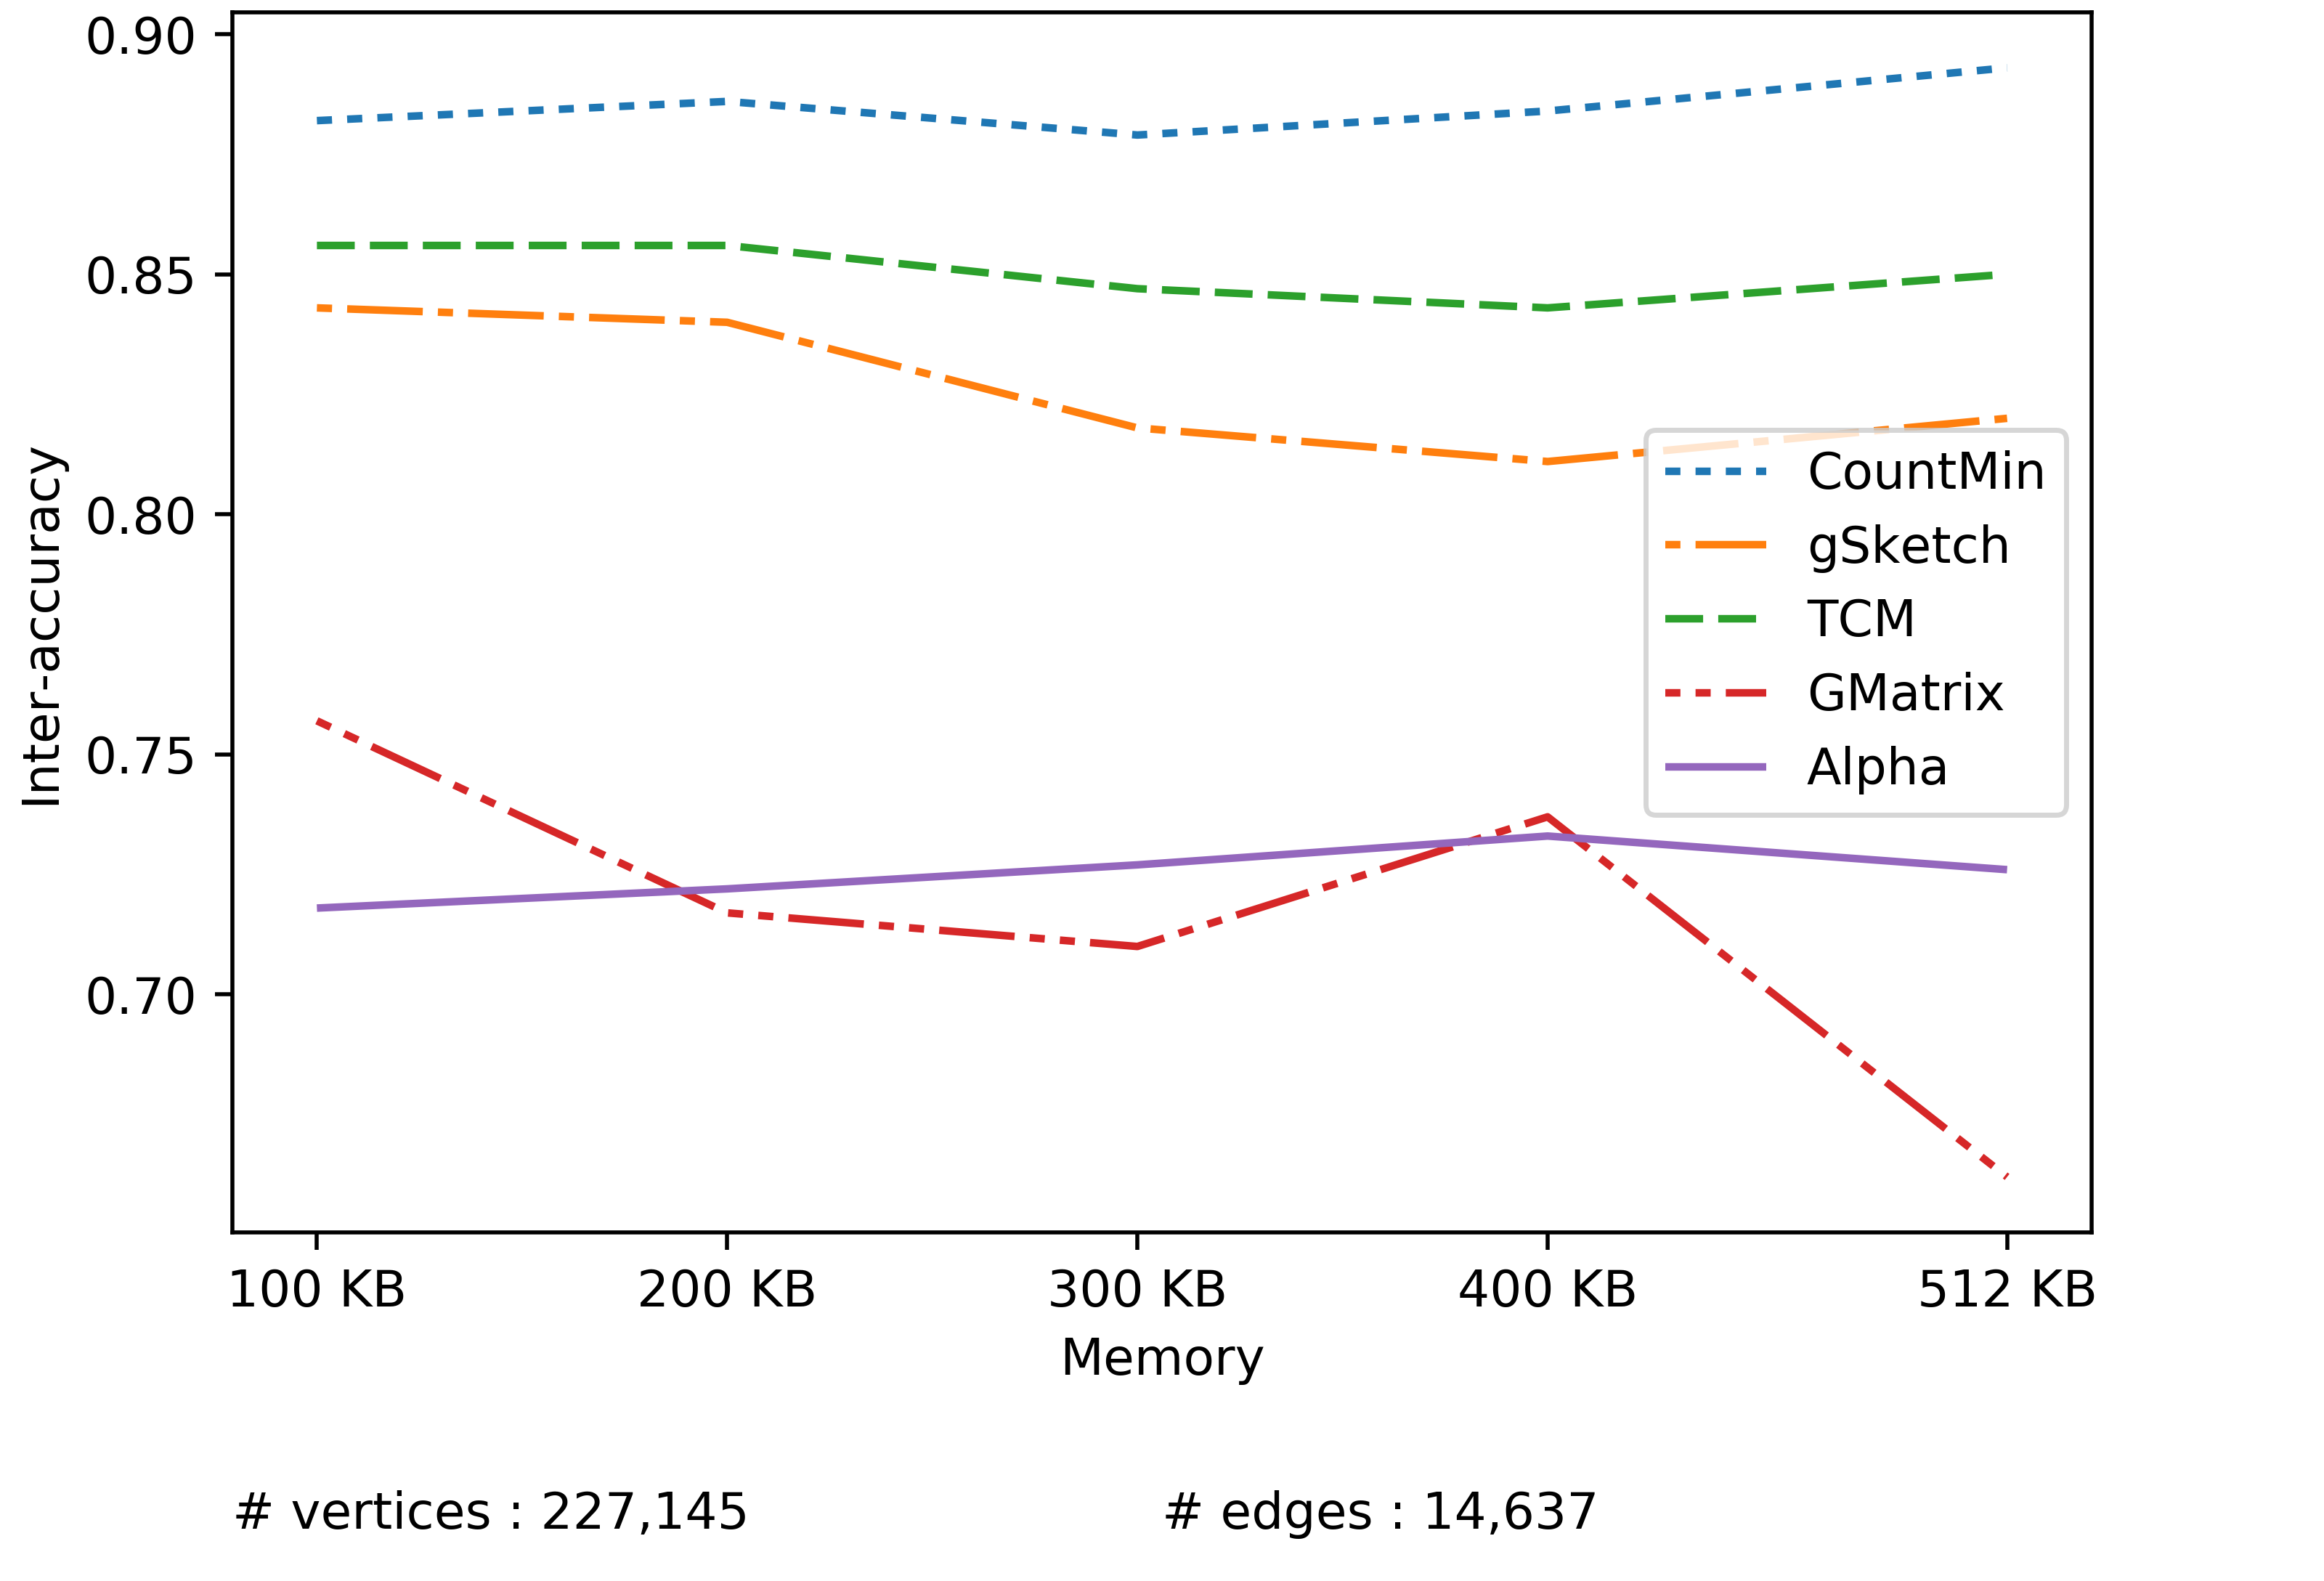
\includegraphics[width=0.85\textwidth]{results/hn/unicorn-wget-hn}
    \vspace{-0.5cm}
    \caption{Inter accuracy of heavy nodes vs Memory for unicorn-wget dataset}
    \label{fig:unicorn-wget-hn}
\end{figure}

\begin{figure}[H]
    \centering 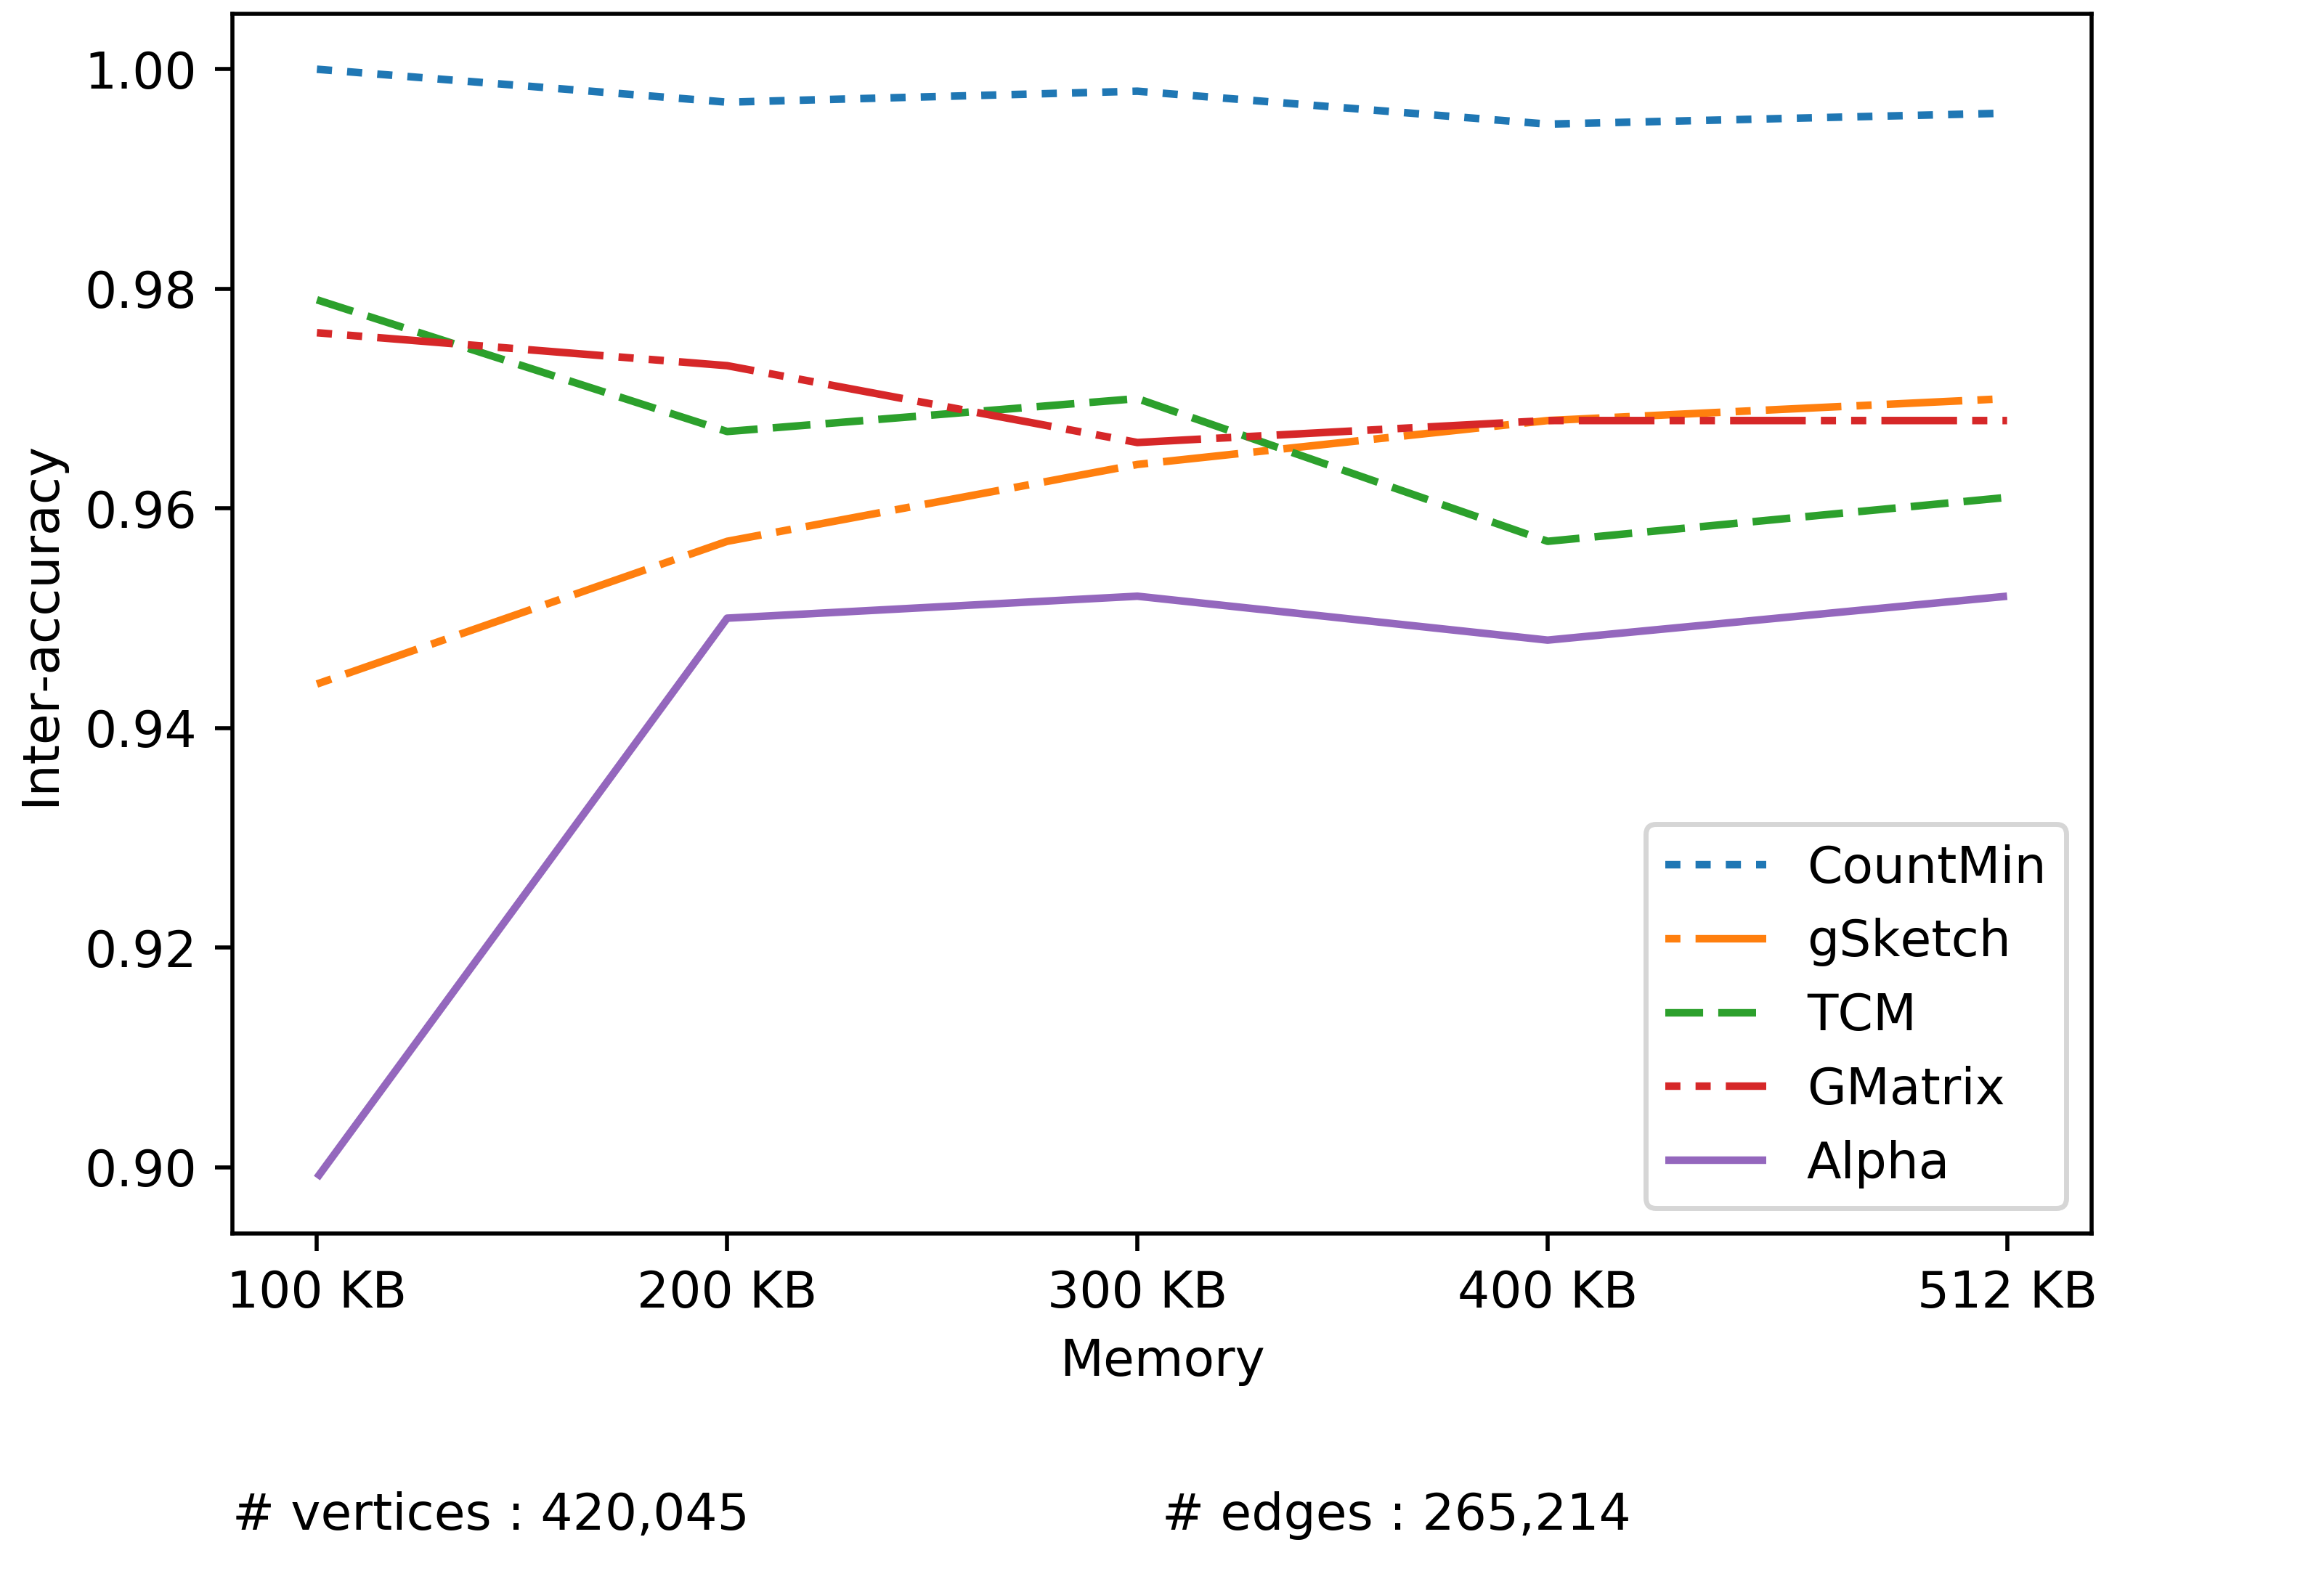
\includegraphics[width=0.85\textwidth]{results/hn/email-EuAll-hn}
    \vspace{-0.5cm}
    \caption{Inter accuracy of heavy nodes vs Memory for email-EuAll dataset}
    \label{fig:email-EuAll-hn}
\end{figure}

\begin{figure}[H]
    \centering 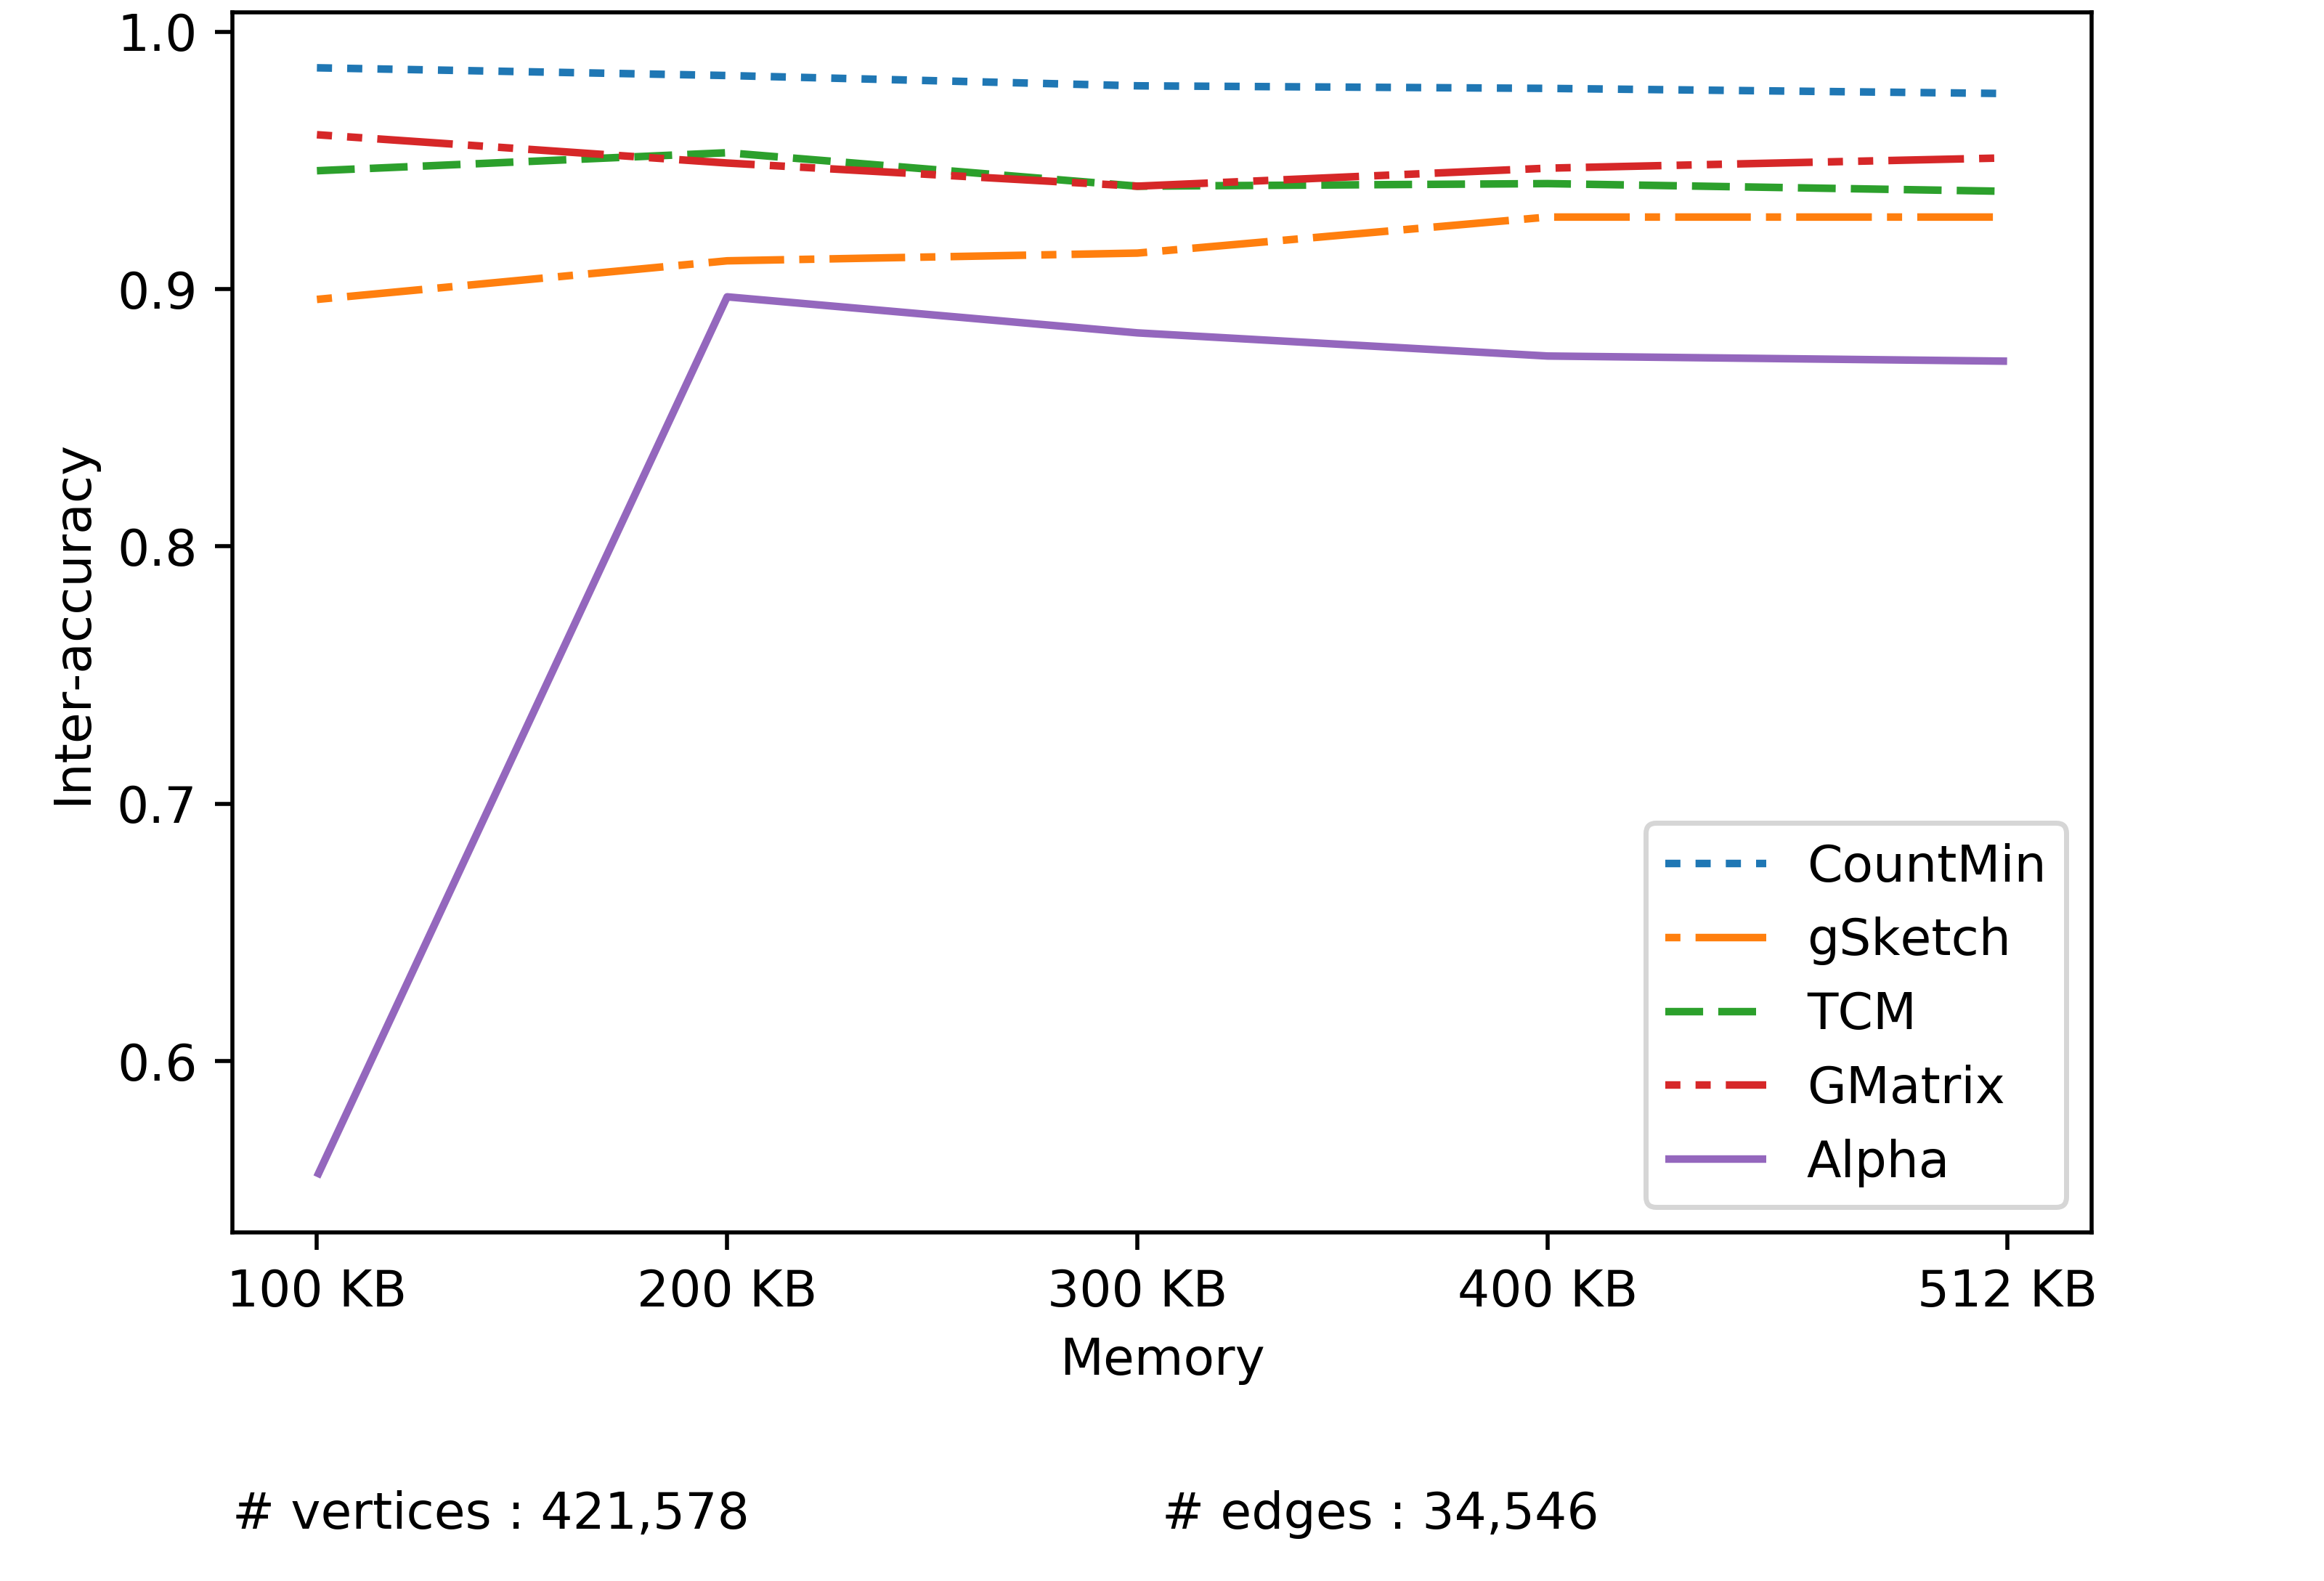
\includegraphics[width=0.85\textwidth]{results/hn/cit-HepPh-hn}
    \vspace{-0.5cm}
    \caption{Inter accuracy of heavy nodes vs Memory for cit-HepPh dataset}
    \label{fig:cit-HepPh-hn}
\end{figure}

\begin{figure}[H]
    \centering 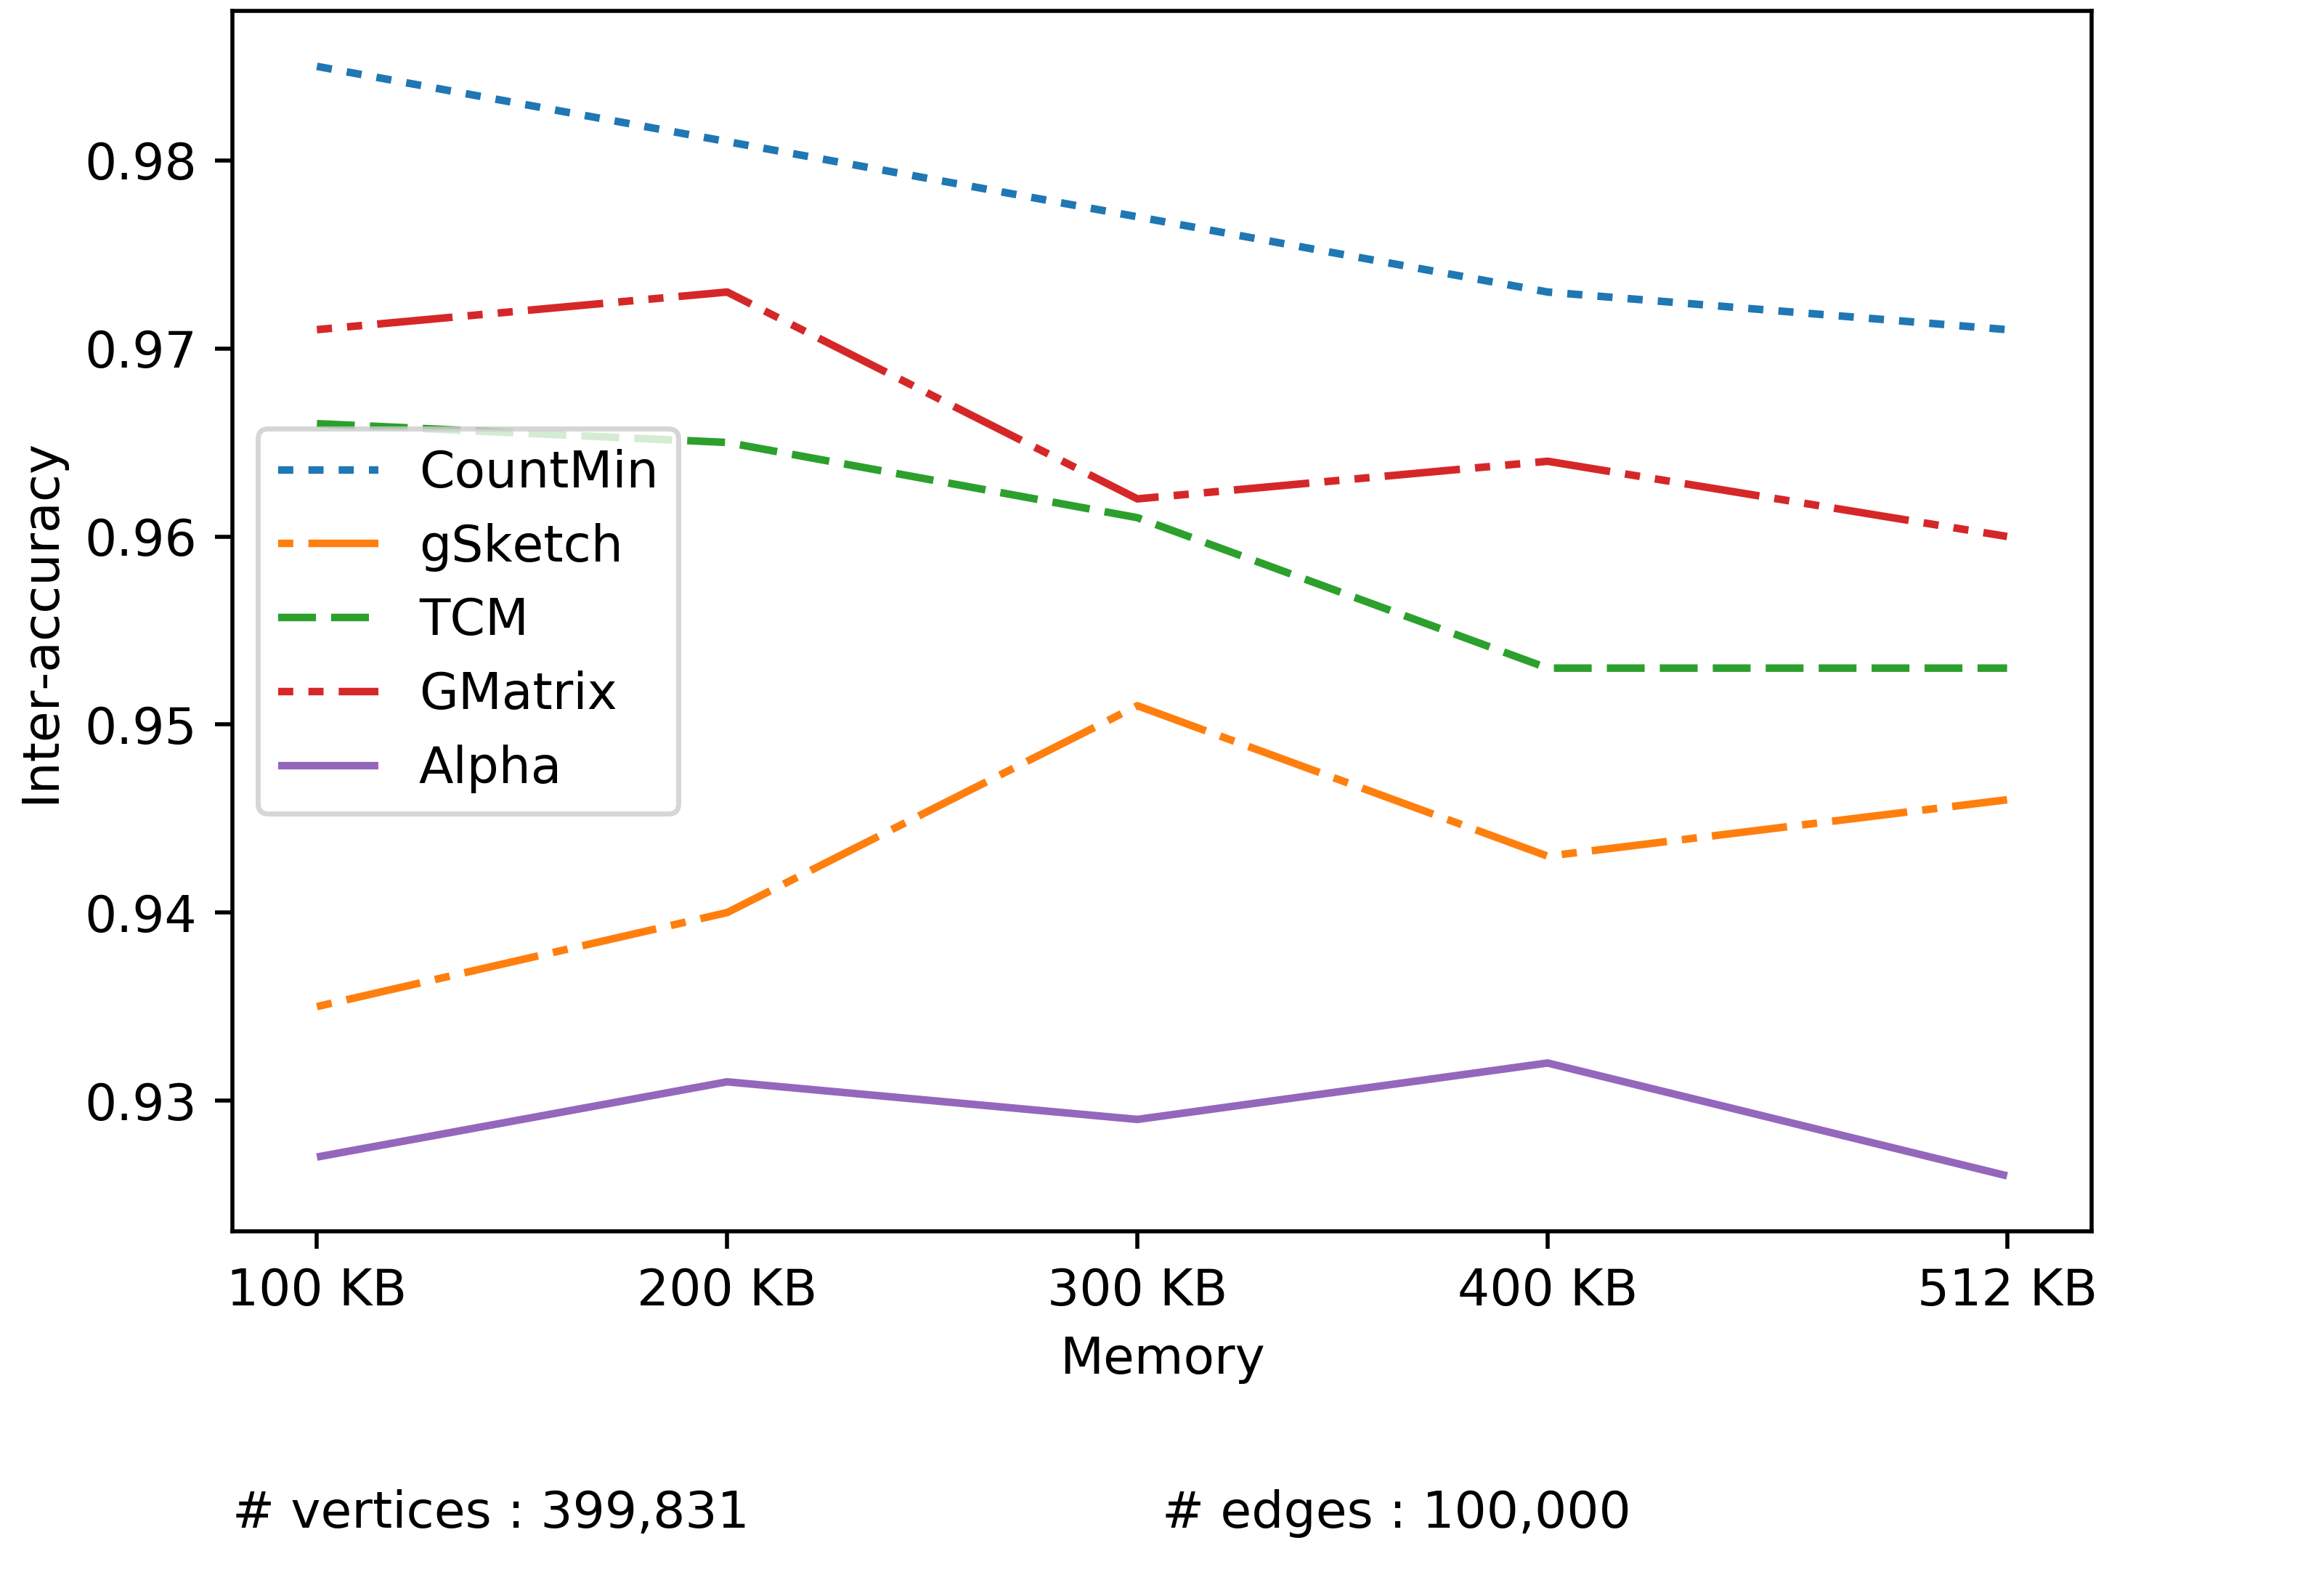
\includegraphics[width=0.85\textwidth]{results/hn/gen-scale-free-hn}
    \vspace{-0.5cm}
    \caption{Inter accuracy of heavy nodes vs Memory for gen-scale-free dataset}
    \label{fig:gen-scale-free-hn}
\end{figure}

\begin{figure}[H]
    \centering 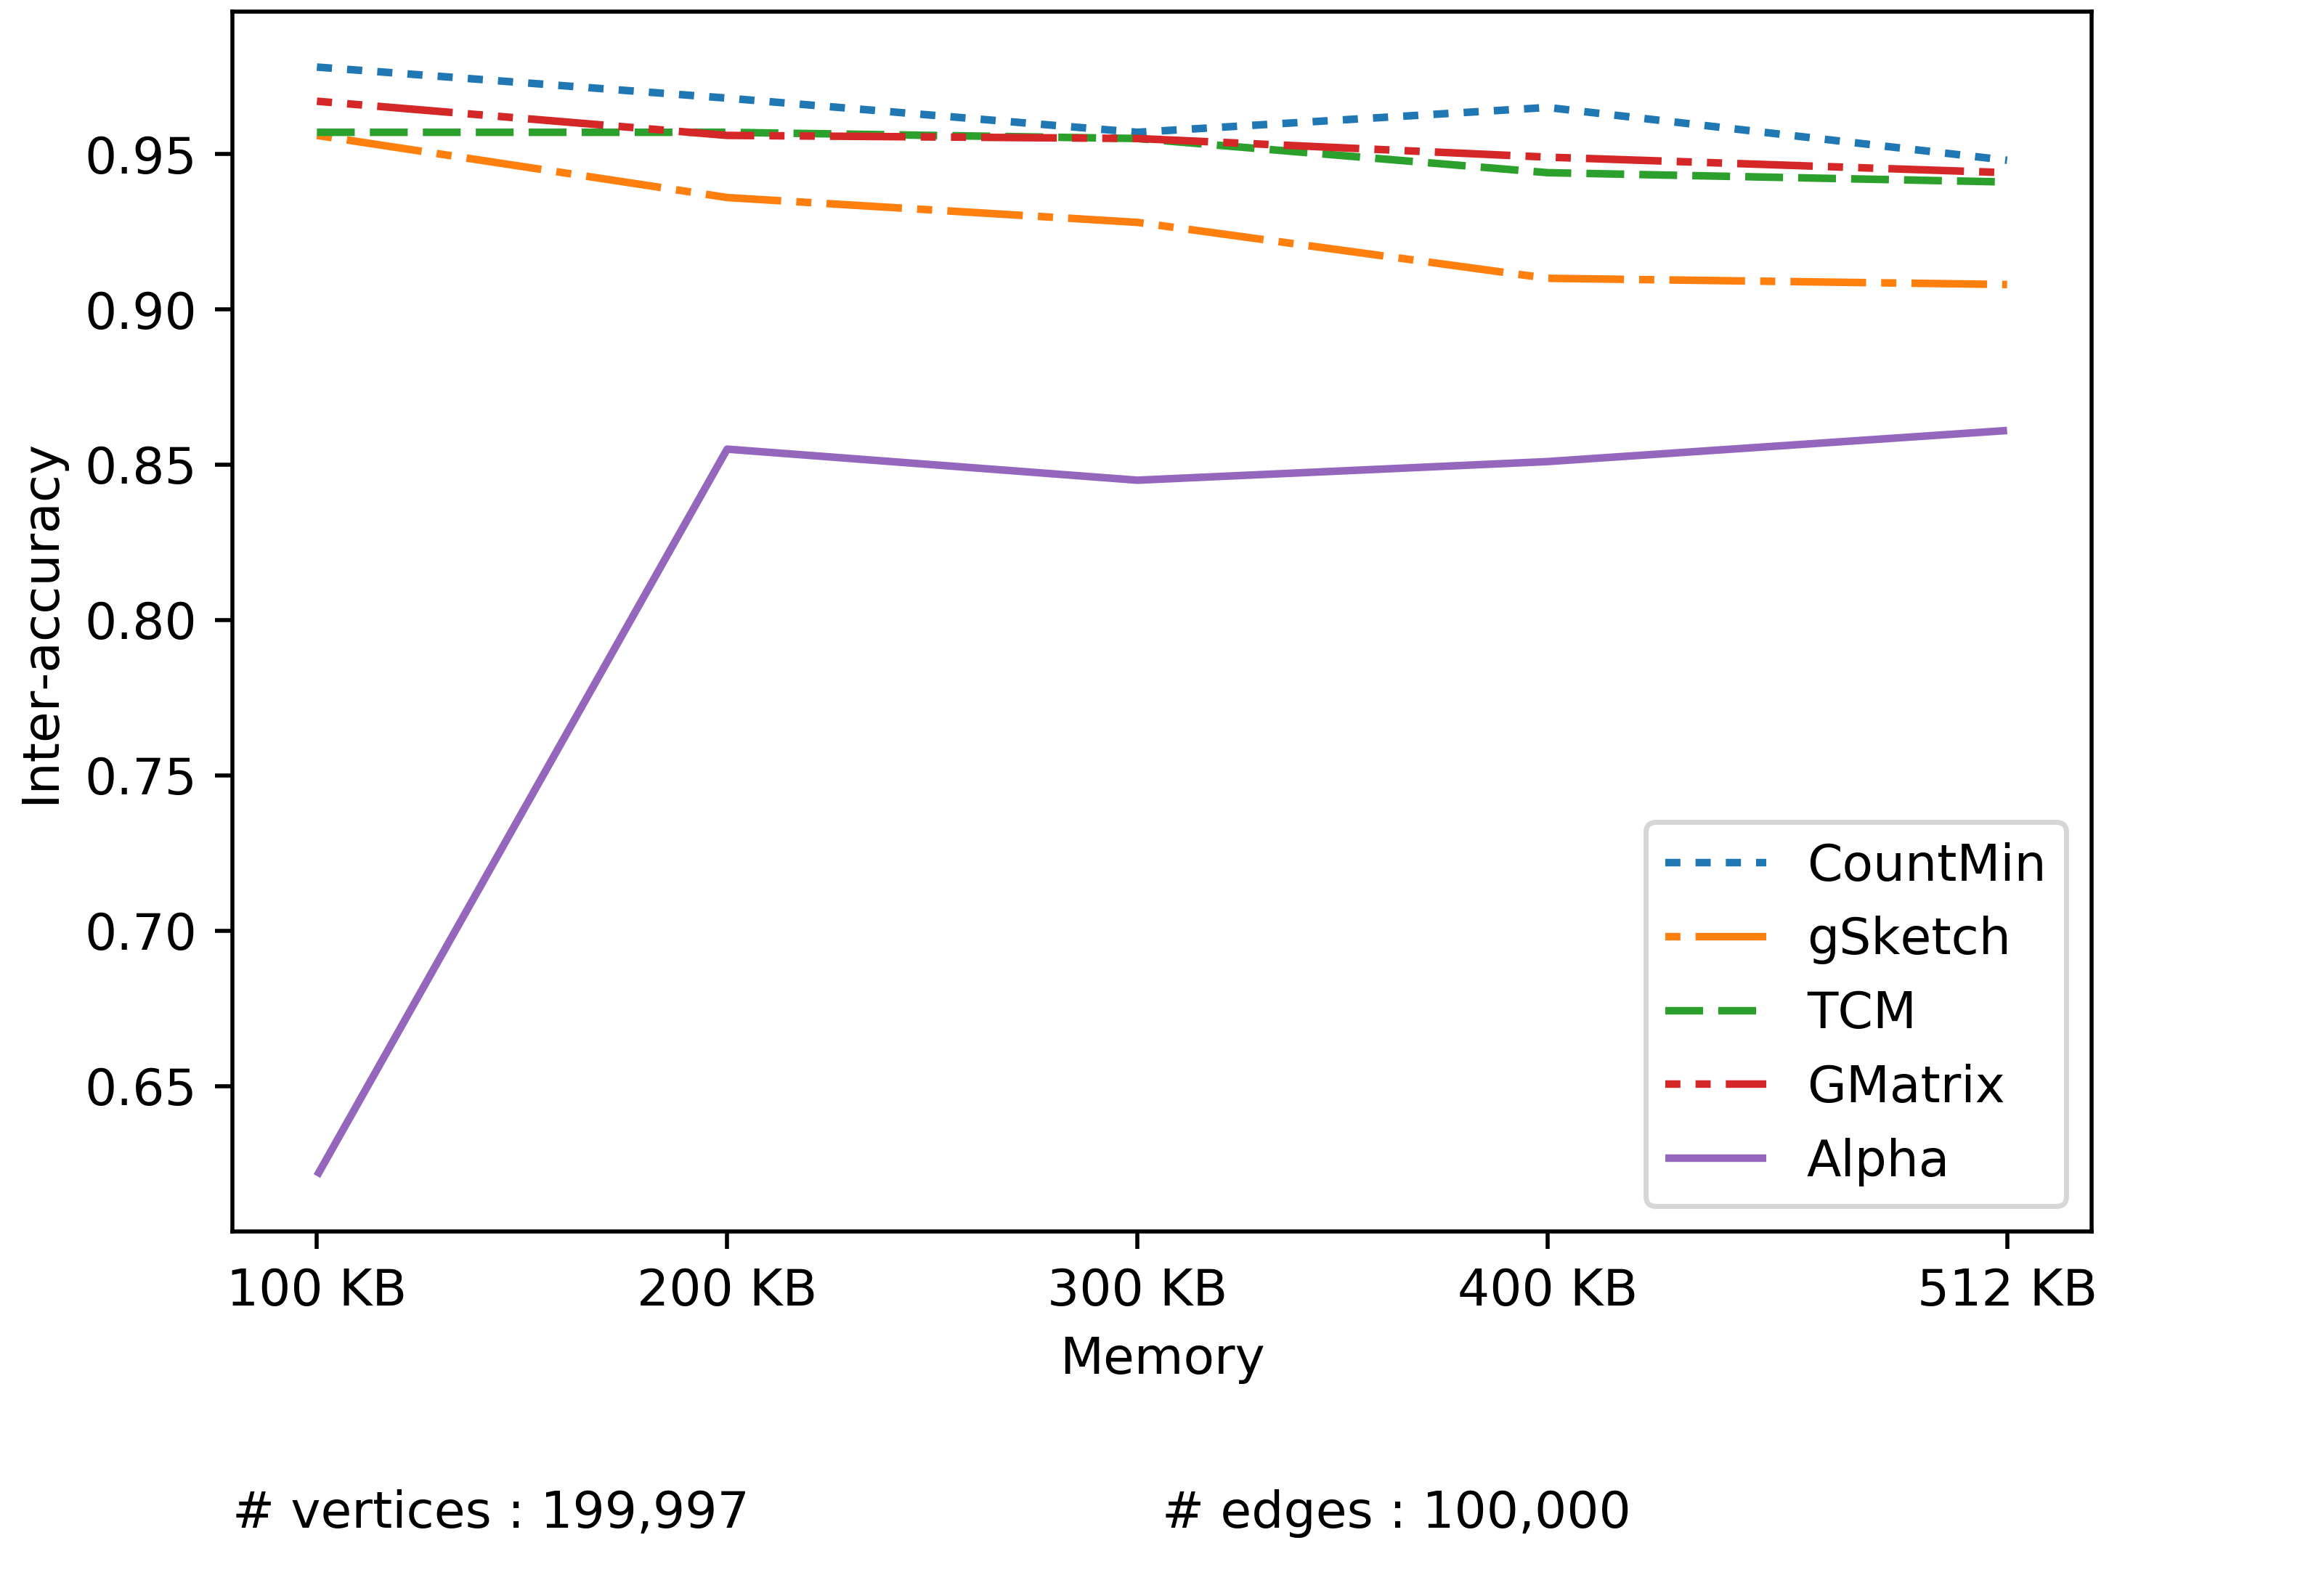
\includegraphics[width=0.85\textwidth]{results/hn/gen-small-world-hn}
    \vspace{-0.5cm}
    \caption{Inter accuracy of heavy nodes vs Memory for gen-small-world dataset}
    \label{fig:gen-small-world-hn}
\end{figure}

\subsection*{Observations and inferences}

\paragraph{}
Both the partitioned sketches, gSketch and Alpha has shown comparably low inter accuracies for top-k heavy node queries for the datasets, unicorn-wget in \autoref{fig:unicorn-wget-hn}, email-EuAll in \autoref{fig:email-EuAll-hn}, cit-HepPh in \autoref{fig:cit-HepPh-hn}, gen-scale-free in \autoref{fig:gen-scale-free-hn} and gen-small-world in \autoref{fig:gen-small-world-hn}. Thus we can infer that the partitioning of the sketches has negatively affected the performance of heavy node queries.

\paragraph{}
CountMin sketch has a higher accuracy for heavy node queries for all the datasets that were tested.

\paragraph{}
The proposed solution Alpha, nor the gSketch are good candidates for heavy node queries. It is evident that the partitioning of the sketches has vastly changed the degree distribution of the original graph, relative to the other sketching techniques. CountMin is best suitable for these types of queries where the heavy node status of the initial graph stream must be preserved.